\subsection{Single Responsibility Principle}
    This principle states that there every class should have a single responsibility
    and there should never be more than one reason to change the class. 
    The code base is sub divided in to 8 packages so that the  and they are:
    \newpage
    \textbf{Project Package description}
    \begin{enumerate}
        \item 
            \textbf{constants} 
                this package contains constants like the Raspberry pi pin 
                numbers, API endpoints. All the variable which will not 
                change and could be used in the project are normally kept here.
        \item 
            \textbf{presenters} 
                This package contains the presenters for the model and the view.
                The class Navigation Manager is here which is responsible to communicate
                with the view and all the three services (I/O service, GPS service and 
                Direction API Service).  
        \item 
            \textbf{customExceptions}
                This package would contain custom exceptions if created.
        \item 
            \textbf{Interfaces}
                This package contains all the Interfaces for the corresponding classes. 
        \item 
            \textbf{listners}
                This package contains custom asynchronous android listeners which gets 
                called when the task get done. For example a listener also known as the
                observer pattern \cite{Hotop2015} to get the result
                from the google API server is also here. It is the most common way of
                making asynchronous calls in android.
        \item 
            \textbf{models}
            This package contains the data layers mainly 
            \href{https://spring.io/understanding/POJO}  {POJO}. Classes defining how the
            data should look like.
        \item 
            \textbf{services} 
                This packages consist of sub packages for the I/O, GPS and Direction service.
        \item 
            \textbf{utils}
                This package has the utilities for making the API requests and other utilities. 
    \end{enumerate}

    \par
        Figure \ref{fig:directionServiceClassDiagram} presents the class diagram
        of the Direction API services. The package Direction Service API is further divided 
        into more packages i.e. Google Direction API service. This package 
        structure is maintained to achieve cohesiveness \cite{AdamCarlson}. Cohesion
        is a way to measure how much a segment in a code belong together. 
        
        \par
        The Google Direction API service contains the actual implementation 
        which make requests to the server and fetches back the result to the 
        presenter \cite{mvp} for further processing. This package is also split up into 
        two concrete implemented class and a abstract interface. The reason
        for splitting them in the manner is again the same to preserve cohesion
        and decoupling which is stated by the Single responsibility principle.
        The classes are explained more in detail in the list below. 
        \begin{enumerate}
            \item 
            \textbf{GoogleDirectionAPIService}
                This class is main class which is exposed to the presenter. It is
                responsible to give the input parameters to the Google direction 
                middleware, run the request in a thread so that the program is not
                blocked using \href{https://developer.android.com/reference/android/os/AsyncTask.html}
                {Async Task Util} this can be found in the util package and the using a listener
                retrieve the results back after the completion of the asynchronous call.
            \item 
            \textbf{GoogleDirectionAPIMiddleware}
                As the name states it this class is a middleware where the instantiation
                of the HTTP client framework \href{http://square.github.io/retrofit/} 
                {Retrofit} and configuration is being done. It is responsible
                to interface between the google API server and the client.
                This class is separated to ensure cohesiveness and decoupling.
            \item 
            \textbf{IGoogleDirectionApiService}
                This is an interface for the Retrofit framework which defines the input
                parameter to carry out the HTTP request to the server.
        \end{enumerate} 

        % Write about why I decided about the two classes and how single responsibility is behind this decision  \ref{fig:directionServiceClassDiagram} 
    \begin{figure}[htbp!]
        \centering 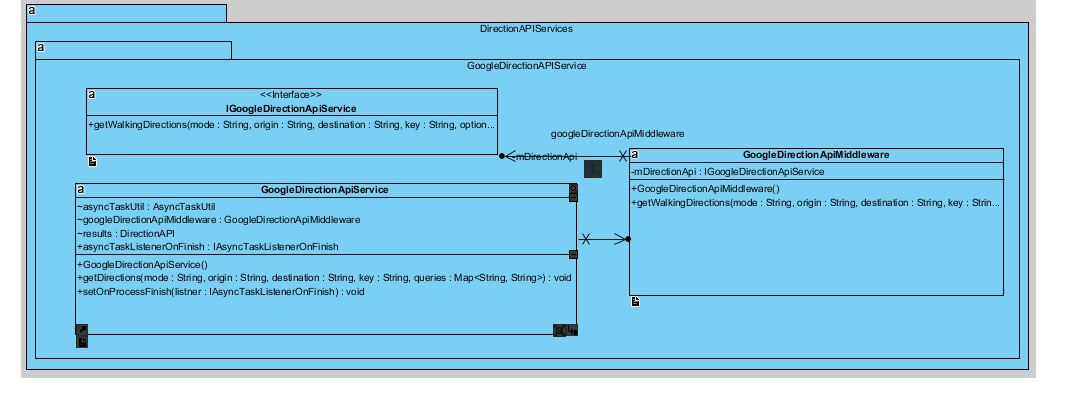
\includegraphics[scale=0.6]{grafiken/directionService.jpg}
        \caption{Class Diagram: Design of the Direction API service}
        \label{fig:directionServiceClassDiagram}
    \end{figure}